\documentclass{entcs} 
\usepackage{entcsmacro}
\usepackage{graphicx}
\newcommand{\Nat}{{\mathbb N}}
\newcommand{\Real}{{\mathbb R}}
\def\lastname{WANG, GUPTA}
\usepackage{picinpar}
\begin{document}
\begin{frontmatter}
\title{Provably Correct Code Generation: A Case Study}\author{Qian
Wang\thanksref{ALL}
\thanksref{qianemail}, Gopal Gupta
\thanksref{gopalemail}}
\address{Department of Computer Science\\University of Texas at Dallas\\
Richardson, TX 75083, USA}
\thanks[ALL]{The authors have been partially
supported by NSF grants  CCR 9900320, CCR 9820852, INT 9904063, by the Department of Education
and the Environmental Protection Agency.}
\thanks[qianemail]{Email:
\href{mailto:qxw015000@utdallas.edu} {\texttt{\normalshape
    qxw015000@utdallas.edu}}} \thanks[gopalemail]{Email:
\href{mailto:gupta@utdallas.edu} {\texttt{\normalshape
     gupta@utdallas.edu}}}


%\thanks[ALL]{Thanks
% to everyone who should be thanked} \thanks[myemail]{Email:
% \href{mailto:myuserid@mydept.myinst.myedu} {\texttt{\normalshape
%     myuserid@mydept.myinst.myedu}}} \thanks[coemail]{Email:
% \href{mailto:couserid@codept.coinst.coedu} {\texttt{\normalshape
%     couserid@codept.coinst.coedu}}}

\begin{abstract}
Provably correct compilation is an important aspect
in development of high assurance software systems.
In this paper we present an approach to provably correct compilation
based on {\it Horn logical semantics} of programming languages and partial
evaluation. We also show that continuation semantics can be
expressed in the Horn logical framework, and
introduce Definite Clause Semantics.
We illustrate our approach by developing
the semantics for the SCR specification language, and using
it to (automatically) generate target code in a provably
correct manner.
\end{abstract}
\begin{keyword}
Horn logic, Denotational Semantics. Compilation
\end{keyword}
\end{frontmatter}

\section{Introduction}

Assuring the correctness of the compilation process
is an important consideration in construction of 
reliable software. If the compiler generates code
that is not faithful to the original program code of
a system, then all our efforts spent in proving the correctness of
the system are futile. Proving that target code 
is correct w.r.t. the program source is especially important
for high assurance systems, as unfaithful target code can 
lead to loss of life and/or property.
Considerable research has been done in this area, starting
from the work of McCarthy \cite{mccarthy}. Most efforts directed
at proving compiler correctness fall into three categories:

\begin{itemize}
\item Those that treat the compiler as just another program and
use standard verification techniques to manually or semi-automatically
establish its correctness. These techniques typically 
employ known mathematical techniques such
as induction proofs, axiomatic semantics, etc. They may
also use theorem provers or advanced reasoning systems
to semi-automate the process. The weakness of this approach 
is that part of the process is manual and may introduce errors.
Another weakness is that each compiler developed
for each language has to be separately proved correct.
\item Those that {\it generate} the compiler automatically from the
      mathematical semantics of the language. Typically
      the semantics used is denotational. Considerable
      research was done in the 70s and 80s to automatically
      generate compilers from the semantic definition of
      a language.  The automatically generated compilers,
      however, have not been used in practice due to their
      slowness and/or complexity of the code generated.

\item Those that use program transformation systems to
transform source code into target code. This approach is
related to the previous one and expresses the operational
semantics of the language as term rewriting rules. These
term rewriting rules can be treated as a specification for
a compiler, and can be proven correct. Target
code is automatically obtained by applying these term-rewriting rules 
to the source code. The disadvantage in this approach
is that specifying the compiler operationally can be
quite a lengthy process. Also, the compilation time can
be quite large since a term-rewriting system will be used
for executing these rules.
\end{itemize}
      
\noindent 
%The last two approaches can be completely
%      automated. in that we have to prove the correctness
%      of the system that generates the compiler from
%      the semantics only {\it once}, and once this is done, 
%      a provably correct compiler for any language can be 
%      generated from its formal semantics.

In this paper we develop an approach based on partial evaluation 
and a type of semantics called {\it Horn logical semantics}.
Our approach is similar in spirit to semantics-based
approaches, however, its basis is Horn-logical
semantics \cite{logden} which possesses 
both an operational as well as 
a denotational (declarative) flavor. 
In the Horn logical semantics approach, both
the syntax and semantics of a language is specified
using Horn logic statements (or pure Prolog \cite{prolog}). The
semantics can be viewed dually as operational or 
denotational. Taking
an operational view, one immediately obtains an
interpreter of the language ${\cal L}$ 
from the Horn-logical semantic description of 
the language ${\cal L}$. Given a program ${\cal P}$ written
in language ${\cal L}$, the interpreter obtained for ${\cal L}$ 
can be used to execute the program. Moreover, given
a partial evaluator for pure Prolog, the interpreter
can be {\it partially evaluated} w.r.t. the program
${\cal P}$ to obtain compiled code for ${\cal P}$.
Since the compiled code is obtained automatically
via partial evaluation of the interpreter, it is
faithful to the source of ${\cal P}$, provided
the partial evaluator is correct.
The correctness of the partial
evaluator, however, has to be proven only once. The
correctness of the code generation process 
for {\it any} language can be certified, provided the
compiled code is obtained via partial evaluation.

Given that efficient execution engines  have been developed for Horn
Logic (pure Prolog), partial evaluation is relatively fast. Also, 
the declarative nature of the Horn logical semantics allows for
language semantics to be rapidly obtained.

In this paper, we further develop the Horn logical semantics approach
and show that continuation semantics can also be expressed in Horn logic.
Moreover, we also show that in Horn logical semantics not only the
syntax but also the semantics can be expressed using the definite
clause grammar notation. The semantics expressed in the DCG notation
allows for the store argument to be naturally hidden. We also show
that continuation semantics expressed as DCGs can be partially evaluated
w.r.t. a source program to obtain target
code in a provably correct manner.
We illustrate this in the context
of the SCR (software cost reduction) method for specifying
embedded real-time systems.
We assume that
the reader is familiar with denotational semantics,
partial evaluation, logic programming,
Prolog and definite clause grammars (\cite{schmidt,jones,prolog}
are good references for these topics).

\section{Horn Logical Semantics}

The denotational semantics of
a language $\cal L$ has three components:
(i) {\it syntax specification:} maps sentences of $\cal L$ to
parse trees; it is commonly specified as a grammar in the BNF format;
(ii) {\it semantic algebra:} represents the mathematical objects used
for expressing the meaning of a program written in the language $\cal L$\/;
these mathematical objects typically are sets or domains (partially
ordered sets, lattices, etc.)
along with associated operations to manipulate the elements of the
sets;
(iii)
{\it valuation functions:} these are functions mapping
parse trees  to elements of the semantic algebras.

Traditional denotational definitions express syntax as BNF grammars,
and the semantic algebras and valuation functions using $\lambda$-calculus. 
In Horn Logical semantics, Horn-clauses (or pure Prolog) and constraints
are used instead to specify all the components of the denotational
semantics of programming languages \cite{logden}. 
There are three major advantages of using Horn clauses and constraints 
for coding denotational semantics.

First, the syntax specification trivially yields an executable parser. 
The BNF specification of a language ${\cal L}$ can be quite easily transformed to a
{\it Definite Clause Grammar} (DCG) \cite{prolog}. 
The syntax specification written in the DCG notation serves as 
a parser for ${\cal L}$. This
parser can be used to parse programs written in ${\cal L}$ and obtain
their parse trees (or syntax trees). 
Thus, the syntactic BNF specification of a language is easily
turned into {\it executable syntax} (i.e., a parser). Note that
the syntax of even context sensitive languages can be specified
using DCGs \cite{killer}.

Second, the semantic algebra and valuation functions of ${\cal L}$ can also be coded
in Horn-clause Logic. Since Horn-clause Logic or pure Prolog is a declarative
programming notation, just like the $\lambda$-calculus, the 
mathematical properties of denotational semantics are preserved.
%This is because logic programming is a declarative programming paradigm
%based on relations, and relations subsume functions (the basis of 
%$\lambda$-calculus). 
Since both the syntax and semantic part of the denotational
specification are expressed as logic programs, they are both
executable. These syntax and semantic  specifications  can
be loaded in a logic programming system and executed, given a program
written in $\cal L$. This provides us with an
interpreter for the language $\cal L$\/. 
In other words, the  {\it denotation}\footnote{We refer to 
the denotation of a program under the Horn-logical semantics as its {\it Horn logical
denotation.}} of a program
written in $\cal L$ is executable. This executable denotation can
also be used for many applications, including automated generation
of compiled code.

Third, non-deterministic\footnote{Non-deterministic in the logic programming
sense.} semantics can be given to a language w.r.t.
resources (e.g., time, space, battery power) consumed during execution. For
example, some operations in the semantic algebra may be specified in multiple
ways (say in software or in hardware) with each type of specification resulting
in different resource consumption. 
Given a program and bounds on the resources that can
be consumed, only some of the many possible semantics may be viable for that
program. Resource bounded partial evaluation \cite{debray} can be used to
formalize resource conscious compilation (for example, energy aware compilation)
\cite{guptawang} via Horn Logical semantics.

Horn-logical semantics can also be used for automatic verification and
consistency checking \cite{logden,ieee}. We do not elaborate any further
since we are not concerned with verification in this paper.

\begin{figwindow}[1,l,%
\fbox{\begin{minipage}[b]{.52\textwidth}
{\tt

Program ::= C.

C ::= C1;C2 |

~~~~~loop while B C end while |

~~~~~if B then C1 else C2 endif |

~~~~~I := E

E ::= N | Identifier | E1 + E2 |

~~~~~E1 - E2 | E1 * E2 | (E)

N ::= 0 | 1 | 2 | ... | 9

Identifier ::= w | x | y | z
}\end{minipage}},%
{BNF grammar \label{gram}}]
In \cite{logden} we show how both the syntax and semantics of a simple imperative language
(a simple subset of Pascal whose grammar is shown in Figure \ref{gram}) can be
given in Horn Logic. The Horn logical semantics automatically yields an
interpreter. Given a program $P$, the interpreter can be partially evaluated w.r.t.
$P$ to obtain $P$'s compiled code.

A program and its corresponding code generated via partial evaluation is shown below.
Note that the semantics is written under the assumption that the program takes exactly
two inputs (found in variables {\tt x} and {\tt y}) and produces exactly one output
(placed in variable {\tt z}).
\end{figwindow}

\begin{verbatim}
    w = x;                          main(X,Y,A) :-
    loop while w > 0                    initialize\_store(B),
       z = z * y ;                      update(a,X,B,C),  
       w = w - 1                        update(b,Y,C,D), 
    end while.                          update(z,1,D,E),
                                        access(x,E,F),    
                                        update(w,F,E,G),
                                        commandwhile(G,H),
                                        access(z,H,A).
          
                                    commandwhile(A,B) :- 
                                       access(w,A,C),
                                          (0<C -> 
                                            access(z,A,D), 
                                            access(y,A,E), 
                                            F is D*E, 
                                            update(z,F,A,G),
                                            access(w,G,H), 
                                            I is H-1, 
                                            update(w,I,G,J),
                                            commandwhile(J,B)
                                          ; B=A ).
\end{verbatim}

Notice that in the program that results from partial evaluation,  
only a series of memory {\tt access}, memory {\tt update}, arithmetic and comparison 
operations are left, that correspond
to {\tt load}, {\tt store}, arithmetic, and comparison 
operations of a machine language. 
The while-loop, whose meaning was expressed using recursion, will
(always) partially
evaluate to a {\it tail-recursive} program.
These tail-recursive calls
are easily converted to iterative structures using jumps.  
Though, the compiled code generated is in Prolog syntax,
true machine code is only a few simple steps away.
The code generation process is provably correct, since target code
is obtained automatically
via partial evaluation. Of course, we need to ensure that the
partial evaluator works correctly. However, this needs to be
 done only once.  Note that once
we prove the correctness of the partial evaluator, compiled code
for programs written in any language can be generated as long as
the Horn-logical semantics of the language is given.

\section{Definite Clause Semantics}

Note that in the code generated, the {\tt update}
and {\tt access} operations are parameterized on the 
memory store (i.e., they take an input store and produce
an output store). Of course, real machine instructions
are not parameterized on store.
This problem can be solved by using the DCG notation
for expressing the valuation predicates as well.

All valuation predicates take a store
argument as input, modify it per the semantics of the
command under consideration and produce the modified
store as output \cite{logden}. Because
the semantic rules are stated compositionally, the
store argument ``weaves" through the semantic
sub-predicates called in the rule. This suggests,
we can express the semantic rules in the DCG notation.
Thus, we can view the semantic rules as computing
the {\it difference} between the output and the input
stores. This difference reflects the effect of the
command whose semantics is being given. Expressed in
the DCG notation, the store argument is hidden
away. For example, in the DCG notation the valuation predicate 

\begin{verbatim}
command(comb(C1,C2),Store,Outstore):- 
    command(C1,Store,Nstore),command(C2,Nstore,Outstore).
\end{verbatim}

\noindent
is written as:

\begin{verbatim}
command(comb(C1,C2)) --> command(C1), comm(C2).
\end{verbatim}

\noindent The complete semantics of the subset of Pascal
considered earlier is shown below as a DCG.

{\small\tt 
\begin{verbatim}
prog_eval(p(Comm),Vala,Valb,Output)-->update(x,Vala), 
     update(y,Valb),command(Comm),access(z,Output).
command(comb(C1,C2))-->command(C1),command(C2).
command(while(B,C)) -->bool(B,Bval),
     ({Bval = true} -> 
            command(C),command(while(B,C));[]).
command(ce(B,C1,C2))-->bool(B,Bval),
     ({Bval = true} -> command(C1); command(C2)).
command(assign(I,E))-->
     expression(E,Val),update(I,Val). 
expression(add(E1,E2),Result)-->
     expression(E1,Val_E1), 
     expression(E2, Val_E2), 
     {Result is Val_E1+Val_E2}.
expression(sub(E1, E2), Result) --> 
     expression(E1, Val_E1),
     expression(E2, Val_E2), 
     {Result is Val_E1-Val_E2}.
expression(mul(E1, E2), Result) --> 
     expression(E1, Val_E1),
     expression(E2, Val_E2), 
     {Result is Val_E1*Val_E2}.
expression(id(X), Result) --> access(X, Result).
expression(num(X), X) --> [].
bool(greater(E1, E2), Bval) --> 
     expression(E1, Eval1), 
     expression(E2, Eval2), 
     {(Eval1 > Eval2 -> Bval = true; Bval = false)}.
bool(less(E1, E2), Bval) --> expression(E1, Eval1), 
     expression(E2, Eval2), 
     {(Eval1 < Eval2 -> Bval = true; Bval = false)}.
bool(equal(E1, E2), Bval) --> expression(E1, Eval1), 
     expression(E2, Eval2), 
     {(Eval1 = Eval2 -> Bval = true; Bval = false)}.
\end{verbatim}
}

\centerline{Semantics expressed as a DCG}

\medskip

\begin{figwindow}[7,l,%
\fbox{\begin{minipage}[t]{0.35\textwidth}
{\small\tt
main(X,Y,A) :-

~~~~~~update(a,X),  

~~~~~~update(b,Y), 

~~~~~~update(z,1),

~~~~~~access(x,F),    

~~~~~~update(w,F),

~~~~~~commandwhile,

~~~~~~access(z,A).

commandwhile :-

~~~~~(access(w,C),

~~~~~~0<C -> 

~~~~~~~~~access(z,D), 

~~~~~~~~~access(y,E), 

~~~~~~~~~F is D*E, 

~~~~~~~~~update(z,F),

~~~~~~~~~access(w,H), 

~~~~~~~~~I is H-1, 

~~~~~~~~~update(w,I),

~~~~~~~~~commandwhile

~~~~~~~; true).
}\end{minipage}},%
{Store eliminated \label{mixt2}\bigskip}]
Expressed in the DCG notation, the semantic rules 
 become more intuitively
obvious. In fact, these rules
have more natural reading; they can be read as
simple rewrite rules.  Additionally, now
we can partially evaluate this DCG w.r.t. an
input program, and obtain compiled code that
has the store argument hidden. 
The result of partially evaluating this DCG-formatted semantics 
is shown in Figure \ref{mixt2}.
Notice that the store argument weaving through the
generated code shown in the original partially evaluated code is gone.
Notice also that the basic operations (such as comparisons,
arithmetic, assignment, etc.) that appear in the target
code are placed in braces in definite clause semantics,
so that the two store arguments are not
added during expansion to Prolog. 
The constructs
appearing within braces can be regarded as the ``terminal"
symbols in this semantic evaluation, similar to terminal
symbols appearing in square brackets in the syntax specification. In fact,
the operations enclosed within braces are the primitive operations
left in the residual target code after partial evaluation.
(Note, however, that these braces can be eliminated by putting
wrappers around the primitive operations; these wrappers will
have two redundant store arguments that are identical, per the
requirements of the DCG notation. Note also that the {\tt -->}
arrow of the DCG notation was replaced by the {\tt :-} prior to
partial evaluation.)
\end{figwindow}

%In fact, one can also write continuation semantics in DCG
%format. In the definite clause continuation semantics, semantics
%of constructs is given in terms of the {\it differences of parse
%tress} (i.e., difference of the input parse tree and the  command
%continuation's parse tree) \cite{diffsem}. Each semantic predicate
%thus relates an individual construct (difference of two parse trees) 
%to a fragment of the store (difference of two stores).
%The advantage of continuation 
%semantics is that a cleaner, more intuitive declarative semantics can be given to 
%imperative constructs such as exceptions, catch/throw, goto, etc. \cite{schmidt}. Continuation
%semantics is not discussed any further due to lack of space. Details can be found
%elsewhere \cite{diffsem}.

\section{Continuation Semantics}

So far we have modeled only direct semantics \cite{schmidt} using Horn logic. It is well
known that direct semantics cannot naturally model exception mechanisms
and {\tt goto} statements of imperative programming languages.
To express such constructs naturally, one has to resort to continuation semantics.
Continuation semantics are also easily modeled in Horn Logic in the DCG format.
In the definite clause continuation semantics, semantics
of constructs is given in terms of the {\it differences of parse
trees} (i.e., difference of the input parse tree and the  
continuation's parse tree) \cite{diffsem}. 
Each semantic predicate
thus relates an individual construct (difference of two parse trees) 
to a fragment of the store (difference of two stores).
Thus, semantic rules are of the form:

~~~{\tt command(C1, C2, Program, S1, S2) :- ...}

\noindent where the difference of C1 and C2 (say $\Delta C$) represents
the command whose semantics is being given, and the difference
of S1 and S2 represents the store which reflects the incremental
change ($\Delta S$) brought about to the store by the command $\Delta C$. Note that
the {\tt Program} parameter is needed to carry the mapping between
labels and the corresponding command. Each semantic rule thus is
a stand alone rule relating the difference of command lists, $\Delta C$, to
difference of stores, $\Delta S$.  
{\it If we view a program as a sequence of commands then its semantics
can simply be obtained by adding the difference of stores for each command.}
That is, if we view a program $P$ as consisting of sequence of commands:

$P = \Delta C_1 + \Delta C_2 + \dots + \Delta C_n$

\noindent then its semantics $S$ is viewed as a combination of the corresponding
differences of stores:

$S = \Delta S_1 + \Delta S_2 + \dots + \Delta S_n$

\noindent and the continuation semantics simply maps each
$\Delta C_i$ to the corresponding $\Delta S_i$.
Additionally, continuation 
semantics allow for cleaner, more intuitive declarative semantics for
imperative constructs such as exceptions, catch/throw, goto, etc. 
\cite{schmidt}. 
Finally, note that the above semantic rule can also be written in the DCG notation
causing the arguments {\tt S1} and {\tt S2} to become hidden:

~~~{\tt command(C1, C2, Program) --> ...}

\noindent
We do not give details due to lack of space. More details can be found elsewhere 
\cite{diffsem}.  However, we give below the continuation semantics 
of the subset of Pascal considered earlier after extending it with statement 
labels and a {\tt goto} statement.  
Note that the syntax trees are now represented as a list of commands. Each
command is represented in the syntax tree as a pair, whose first element
is a label (possibly null) and the second element is the command itself.
Only the valuation functions for commands are shown (those for expressions,
etc., are similar to the one shown earlier).

{\small\tt
\begin{verbatim}
prog([ ], _, _, 0) --> [ ].
prog(CommList,Val_x,Val_y,Output) -->
     initialize_store, update(x, Val_x), update(y, Val_y),
     comm_list(CommList,CommList), access(z,Output).

comm_list([ ],_) --> [ ].
comm_list(CurrList,Program)-->
    comm(CurrList,Rest,Program), comm_list(Rest,Program).
comm([(_,while(B,LoopBody))|T],T,Program)--> 
    fix(if(B,LoopBody),Program).
comm([(_,ce(B,C1,C2))|T],T,Program) -->
    ((bool(B)) -> comm_list(C1,Program); comm_list(C2,Program)).
comm([(_,ce(B,C))|T],T,Program) -->  
    ((bool(B)) -> comm_list(C,Program); [ ]).
comm([(_,goto(ID))|_],GotoCont,Program)-->
     {find_label(ID,Program,GotoCont)}.
comm([(_,assign(id(I), E))|T],T,_) --> expr(E,Val),update(I,Val). 
comm([(_,abort)|_],[ ],_) --> [ ].

fix(if(B,LoopBody),Program)-->
     ((bool(B))-> comm_list(LoopBody,Program),
                  fix(if(B,LoopBody),Program); [ ]).
\end{verbatim}
}


\noindent
The code for {\tt find\_label/3} predicate is not shown.
It looks for the program segment that is a target of a
{\tt goto} and changes the current continuation to that 
part of the code.  Consider the program shown below to the left:
The result of partially evaluating the interpreter obtained from
the semantics w.r.t. this program 
(containing a {\tt goto}) is shown below to the right.

\begin{verbatim}
   z = 1;                 main(A, B, C) :-
   w = x;                     initialize_store,
   goto L1;                   update(x, A),
   loop while w > 0           update(y, B),
          z = z * y;          update(z, 1),
      L1: w = w - 1           access(x, D),
   endloop while;             update(w, D),
   z = 8.                     access(w, E),
                              F is E-1,
                              update(w, F),
                              fix_ifgreatidw1,
                              update(z, 8),
                              access(z, C).
                         fix_ifgreatidw1 :-
                              (   access(w, A),
                                  0<A ->
                                  access(z, B),
                                  access(y, C),
                                  D is B*C,
                                  update(z, D),
                                  access(w, E),
                                  F is E-1,
                                  update(w, F),
                                  fix_ifgreatidw1
                              ;   true
                              ).
\end{verbatim}

\section{A Case Study in SCR}

We have applied our approach 
to a number of practical applications. 
These include generating code for parallelizing compilers in
a provably correct manner \cite{logden}, 
generating code for controllers specified in Ada \cite{bart}
and for domain specific languages \cite{dsl} in a provably
correct manner, and most recently generating code in a provably
correct manner for the Software Cost Reduction (SCR) framework.
In the rest of the paper, we show that Horn logical
semantics can be practically applied; we apply it to the domain
specific language of SCR, discussed next.

The SCR (Software Cost Reduction) requirements method is a software development 
methodology introduced in the 80s \cite{Heninger78} for engineering reliable software systems. 
The target domain for SCR is real-time embedded systems.  
The SCR method has been extended to describe not only functional requirements (the values the 
system assigns to outputs) but also nonfunctional (e.g., timing and accuracy) requirements. 
A number of  automatic tools have been developed to aid in formal specification, verification and 
validation of systems using the SCR method \cite{Constance96}. 
SCR has been applied to a number of practical systems, including avionics system (the A-7 
Operational flight Program), a submarine communication system, and 
safety-critical components of a nuclear power plant \cite{Constance96}. The SCR method 
is scalable and has been applied to document requirements of the Lockheed's 
C-130J Operational Flight Program which resulted in 
approximately 100,000 lines of Ada code.  
%While a number of tools have been
%developed for checking consistency of an SCR specification, generation of executable code
%in a provably correct manner is a major problem affecting reliability.

The SCR method describes system behavior by a mathematical relation between monitored variables and controlled 
variables. This relation is concisely specified using {\it condition}, {\it events} and 
{\it tables}. A condition is a predicate 
defined on one or more variables in the specification. An event occurs when any variable changes values. 
The environment changes monitored values and causes input events. In response, the system updates 
the value of one or more controlled variable according to some relations.
Each SCR table specifies the required value of a variable as a mathematical function defined on conditions 
and events. There are three kinds of table used in SCR: {\it condition} tables, {\it event} tables, and {\it mode 
transition} tables. The tables facilitate industrial application of the SCR method since engineers
find tables relatively easy to understand and to develop \cite{Constance96}. In additional, tables 
can describe large quantities of requirement information concisely.

\subsection{The Four-Variable Model}

There are several versions of SCR. One of the most important versions is the Four Variable Model. 
The Four Variable Model \cite{FAULK89}, illustrated in Figure \ref{actual4}, represents requirements 
as a set of mathematical relations on four sets of variables (monitored, controlled, input, 
and output variables). A monitored variable 
represents an environmental quantity that influences system behavior, while a controlled variable represents
an environmental quantity the system controls. A black box specification of required behavior is given as two relations 
(REQ and NAT) from the monitored quantities to the controlled quantities (rather than inputs to outputs). NAT,
which defines the set of possible values, describes the natural constraints on the system behavior, 
such as constraints imposed by physical laws and the system environment. REQ defines the additional 
constraints on the system to be built as relations the system must maintain between the monitored and 
the controlled quantities \cite{Constance96}. 

\begin{figure}
\begin{center}
  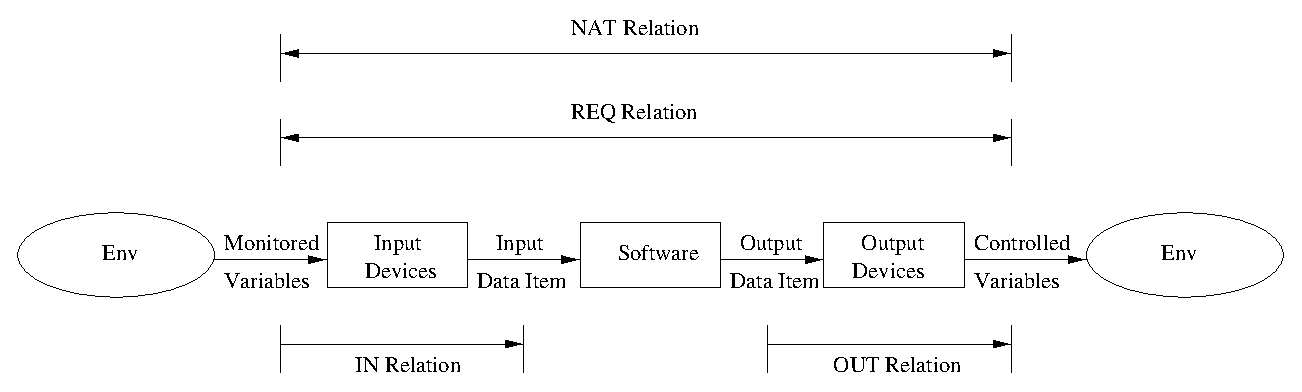
\includegraphics[height=1.8in,width=5in]{fig5.eps}
  \caption{The Four-Variable Model}
  \label{actual4}
\end{center}
\end{figure} 

%\begin{figure*}[htb]
%\centerline{\psfig{figure= fig5.eps,width=0.75\textwidth}}
%\caption{The Four-Variable Model}
%\label{actual4}
%\end{figure*}

A domain specific language \cite{Elizabeth02} has been designed to write SCR specifications
using the four variable model, as well as a large number of tools have been developed to
help in checking consistency of the requirement specifications \cite{Constance96}. 
While the consistency of requirement specifications can be checked using these tools, a 
hurdle still remains in having absolute confidence in the final system obtained. This hurdle
pertains to ensuring that the compilation process is provably correct, i.e., after
consistency checking, when the
SCR specification is translated into executable code then making sure that 
the code generated is faithful to the original specification.

We have applied our method discussed in this paper to overcome this hurdle.
A Horn logical semantics for the SCR domain specific language was developed.
This semantics consists of the syntax specification, semantic algebra and valuation
predicates. The semantic algebra consists of operations for accessing and updating the 
store (values of variables as well as their type) and maintaining the various environments. 
Development of this semantics required just a few weeks of work (a significant
part of this time was spent understanding the SCR method).
The DCG notation was used both for syntax as well as semantics.

The grammar of SCR consists of five sections  (type definitions, constant definitions, 
variable declarations, assumptions and assertions, and function definitions). 
User-defined data types are listed in the type definitions section. 
There are two types of user define data types: (i) enumerated 
type and (ii) integer type associated with a range. 
Variable declarations can include four types of variables:
monitored variables, controlled variables, term variables and mode classes. 
The assumptions and assertions section contains
predicates describing relations between variables, i.e., 
each assumption or assertion is a logical formula. 
The violation of an assumption indicates that the input 
does not obey the assumed environmental constraints. 
If an assertion is violated, it means that the specification 
does not satisfy a property that is was expected to 
satisfy.  Function in SCR are defined by either a 
condition or an event table. Functions are used to 
update values of dependent variables 
when a monitored variable changes. 
The DCG for SCR has been developed in accordance to the BNF grammar supplied to us
by Naval Research Lab researchers. The semantics of SCR's DSL is given 
in terms of the store semantic algebra extended with type information.

\begin{figure}
\begin{center}
  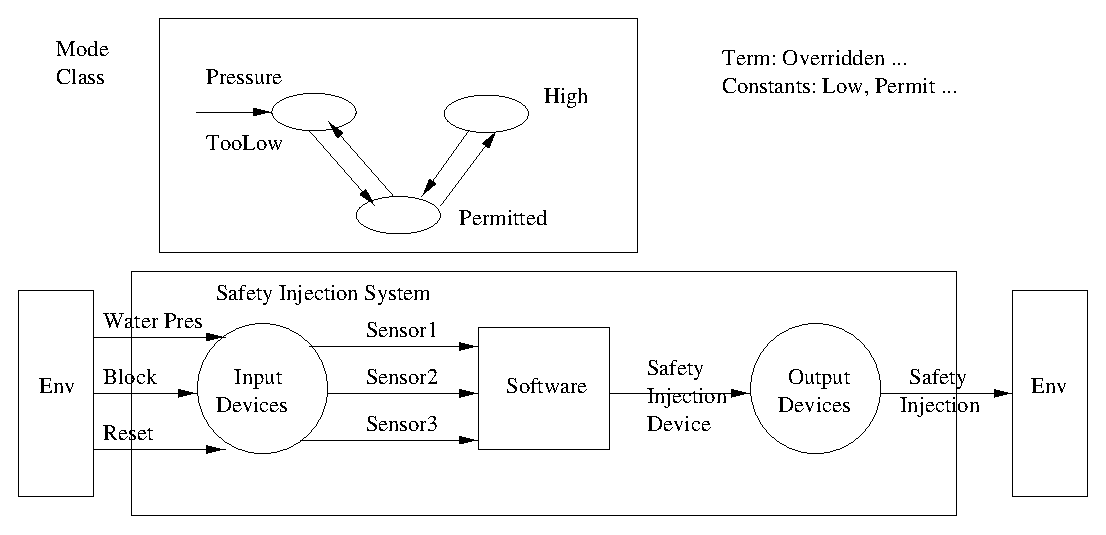
\includegraphics[height=2.1in,width=5.2in]{fig4.eps}
  \caption{Requirements Spec. for Safety Injection}
  \label{actual5}
\end{center}
\end{figure} 

%\begin{figure*}[htb]
%\centerline{\psfig{figure= fig4.eps,width=0.75\textwidth}}
%\caption{Requirements Spec. for Safety Injection}
%\label{actual5}
%\end{figure*}

To illustrate generation of code for SCR in a provably correct manner, 
we consider a simplified version of the control system for safety injection described 
in \cite{Constance96}. The system uses three sensors to monitor water pressure and adds coolant 
to the reactor core when the pressure falls below some threshold. The system operator blocks safety 
injection by turning on a ``block" switch and resets the system after blockage by turning on a ``reset" 
switch. Figure \ref{actual5} shows how SCR constructs could be used to specify the requirements of the control 
system. Water pressure and the ``block" and ``reset" switches are represented as monitored variables called
{\tt WaterPres}, {\tt Block}, and {\tt Reset}. Safety injection is represented as 
a controlled variable called {\tt SafetyInjection}. Each sensor represents an 
input. The hardware interface between the control system software and the safety injection 
system serves as output. 
A mode class {\tt Pressure} and a term {\tt Overridden} help make the specification of
the safety injection system concise. 
{\tt Pressure} has three modes: {\tt TooLow}, {\tt Permitted}, and {\tt High}. 
A drop in water pressure below a constant {\tt Low} 
causes the system to enter mode {\tt TooLow}; an increase in pressure above a 
larger constant {\tt Permit} causes the system to enter mode {\tt High}.
The term {\tt Overridden} is {\tt true} if safety injection is blocked, it is {\tt false} 
otherwise.  An example of a condition in the specification is {\tt WaterPres < Low}. 
Two examples of events are the input event {\tt event@T(Block=on)}
(the operator turns Block from {\tt off} to {\tt on}) and the conditioned event {\tt @T(Block=On) WHEN 
WaterPres < Low} (the operator turns {\tt Block} to on when water pressure is below 
{\tt Low}). 
The program corresponding to this system written in the SCR domain specific
language was also supplied to us by researchers at the Naval Research Labs and is shown 
in Appendix I. More details 
about SIS can be found elsewhere \cite{Constance96}.


The Horn logical semantics developed for SCR immediately provides us with
an interpreter on which the program above can be executed. Further, the
interpreter was partially evaluated w.r.t. this program using the Mixtus
system, and compiled code
was obtained. The partially evaluated code generated that
corresponds to the safety injection system is shown in Appendix II.
The whole partial evaluation (using definite clause continuation semantics of SCR)
required 27.1 seconds on a Sun Fire 880 with 150 MHz clock-speed
and 1 CPU and 2 GB memory
and generated 367 lines of assembly code in Prolog syntax (shown in Appendix II). 
In \cite{Elizabeth02}, given the same example code (Appendix I), 
a {\it relation-based} strategy (that associates C code as an attribute with
parse tree nodes) required 
20 minutes to generate C code, while
a transformation-based
method using the APTS system  \cite{apts} took four minutes to 
generate 293 lines of C code 
(execution done on a SUN Ultra 450 with 2 
UltraSPARC-II 296MHz CPUS and 2GB memory, running Solaris 5.6 \cite{Elizabeth02}).

Even though our respective experiments have been done on different machines, the machines
are comparable in speed. As can be noticed,
the time taken to generate code in our case is considerably better.
Note that we did not optimize the semantics at all to make it more amenable to partial
evaluation as that would have reduced the readability of the semantics. 

\section{Related Work}

Considerable work has been done in manually or semi-mechanically
proving compilers correct. Most of these efforts are based
on taking a specific compiler and showing its
implementation to be correct. A number of tools (e.g.,
a theorem prover) may be used to semi-mechanize the
proof. Example of such efforts range from McCarthy's work
in 1967 \cite{mccarthy} to more recent ones
\cite{borger,pfenning,sttr}.
As mentioned earlier, these approaches are either 
manual or semi-mechanical, requiring human intervention,
and therefore not completely reliable enough for engineering
high-assurance systems. ``Verifying Compilers" have also
been considered as one of the grand challenge for computing
research \cite{hoare03}, although the emphasis here is more
on developing a compiler that can verify the assertions inserted
in programs (of course, such a compiler has to be proven correct
first). 


Considerable work has also been done on generating compilers
automatically from language semantics \cite{schmidt}.  
However, because the syntax is specified as a (non-executable) BNF and semantics
is specified using $\lambda$-calculus, the automatic generation process
is very cumbersome. The approach outlined in this paper falls in this
class, except that it uses Horn logical semantics which, we believe and
experience suggests, can be manipulated more efficiently.

Considerable work has also been done in using term rewriting systems
for transforming source code to target code. In fact,
this approach has been applied by researchers at NRL to automatically
generate C code from SCR specification using the APTS \cite{apts}
program transformation system. As noted earlier, the time taken is
considerably more than in our approach. Other approaches that fall in
this category include the HATS system \cite{hats} that use tree rewriting
to accomplish transformations. Other transformation based approaches
are mentioned in \cite{Elizabeth02}.

Recently, Pnueli at al have taken the approach of verifying a given
run of the compiler rather than a compiler itself \cite{pnueli}.
This removes the burden of maintaining the compiler's correctness proof; 
instead each run is proved correct by establishing a refinement 
relationship.  However, this approach is limited to very simple languages.
As the authors themselves mention, their approach ``seems to work in all cases that the source
and target programs each consist of a repeated execution of a single
loop body ..,"  and as such is limited. For such simple languages, we believe that
a Horn logical semantics based solution will perform much better 
and will be far easier to develop. Development of the
refinement relation is also not a trivial task. For general programs and general 
languages, the scalability of the approach is not established.

\section{Conclusions}

In this paper we presented an approach based on denotational
semantics, Horn logic, and partial evaluation for obtaining
provably correct compiled code. We illustrated
our approach in the context of the SCR method for specifying
real-time embedded system. The complete syntax and semantic
specification for SCR was developed and used for automatically
generating code for SCR specifications. Our method produces 
executable code considerably faster than other transformation
based methods for automatically generating code for SCR specifications.


\begin{ack}
We are grateful to Constance Heitmeyer and Elizabeth Leonard of the
Naval Research Labs for providing us with the BNF grammar of SCR and
the safety injection program as well as for discussions. 
\end{ack}


\begin{thebibliography}{10}\label{bibliography}
\bibitem{debray}
S. Debray. Resource bounded partial evaluation. PEPM 1997. pp. 179-192.

\bibitem{sttr}
A. Dold, T. Gaul, W. Zimmermann 
Mechanized Verification of Compiler Backends 
Proc. Software Tools for Technology Transfer (STTT'98), 
Aalborg, Denmark, July 12-13, 1998.

\bibitem{FAULK89}
S. R. Faulk. State Determination in Hard-Embedded Systems. Ph.D. 
Thesis, Univ. of NC, Chapel Hill, NC, 1989.

\bibitem{futamura} Y. Futamura. Partial Evaluation of
 Computer Programs: An approach to compiler-compiler.
{\it J. Inst. Electronics and Comm. Engineers, Japan}.
1971.                           

\bibitem{logden}
G. Gupta  ``Horn Logic Denotations and Their Applications,"
{\it The Logic Programming Paradigm: A 25 year perspective}.
Springer Verlag.  1999:127-160.                              

\bibitem{killer}
G. Gupta, H-F. Guo, A. Karshmer, E. Pontelli, et al.
Semantic-Based Filtering: Logic  Programming's Killer App?
4th International Symposium on Practical Aspects of Declarative
Languages, LNCS 2257, Springer Verlag, pp. 82-100, Jan. 2002.


\bibitem{ieee}
G. Gupta, E. Pontelli. A Constraint-based Denotational Approach to
        Specification and Verification of Real-time Systems.
        In {\it Proc. IEEE Real-time Systems Symposium}, 
	pp. 230-239. Dec. 1997.

\bibitem{dsl} G. Gupta, E. Pontelli. 
	A Logic Programming Framework for Specification
	and Implementation of Domain Specific Languages.
	In {\it Essays in Honor of Robert Kowalski}, 2003,
	Springer Verlag LNAI,

\bibitem{Heninger78} K. L. Henninger. Specifying software requirements for complex
	systems: New techniques and their application. IEEE Trans.
	on Software Engineering. SE-5, 1. pp. 2-13.

\bibitem{winskel}
C. Gunter. Programming Language Semantics. MIT Press. 1992.

\bibitem{pfenning} 
J. Hannan, F. Pfenning.
        Compiler Verification in {LF}.
	{\it Proc. Seventh Annual {IEEE} Symposium 
	on Logic in Computer Science}.
	pp. 407--418. 1992.

\bibitem{Constance96}
C. L. Heitmeyer, R. D. Jeffords, and B. G. Labaw. Automated Consistency Checking of 
Requirements Specifications. ACM Trans. Software Eng. and Methodology 5, 3, July 1996.

\bibitem{hoare03} C. A. R. Hoare. The Verifying Compiler: A Grand
	Challenge for Computing Research. J.ACM, 50(1):63-69. Jan 2003.

\bibitem{jones} N. Jones. Introduction to Partial Evaluation.
	In {\it ACM Computing Surveys}. 28(3):480-503.

\bibitem{bart}
L. King, G. Gupta, E. Pontelli. 
	Verification of BART Controller: An Approach based\\
	on Horn Logic and Denotational Semantics.
        In {\it High Integrity Software}, 
	V. Winter and S. Bhattacharya (eds), April 2001,
	Kluwer Academic.

\bibitem{ecce}
M. Leuschel, B. Martens, and D. De Schreye. 
Controlling Generalization and Polyvariance in Partial Deduction of Normal Logic Programs. 
ACM Transactions on Programming Languages and Systems (TOPLAS), 20(1):208-258.

\bibitem{Elizabeth02}
E. I. Leonard and C. L. Heitmeyer. Program Synthesis from Requirements Specifications 
Using APTS. Kluwer Academic Publishers, 2002.

\bibitem{stuckey}
K. Marriott and P. Stuckey.
Constraint Programming. MIT Press, 1998.

\bibitem{mccarthy}
J. McCarthy and J. Painter.
Correctness of a Compiler for Arithmetic Expressions. 
MIT AI Lab Memo, 1967.

\bibitem{Steven98}
S. P. Miller. Specifying the model Logic of a Flight Guidance Systems in CoRE and SCR. 
Pages:44-53 Series Proceeding Article, 1998 

\bibitem{apts} R. Paige. Viewing a Program Transformation System
	at Work. {\it Proc. Programming Language Implementation
		and Logic Programming}, Springer, LNCS 844. 1994.

\bibitem{borger} 
C. Pusch.  Verification of Compiler Correctness for the {WAM}.
{\it Proc 9th International Conference on Theorem Proving 
in Higher Order Logics ({TPHOL}'96)}.
Springer-Verlag LNCS 1125, 1996.

\bibitem{pnueli} 
A. Pnueli, M. Siegel, E. Singerman.  Translation Validation.
{\it Proc TACAS'98}, Springer Verlag LNCS, 1998.


\bibitem{mixtus} D. Sahlin. An Automatic Partial 
	Evaluator for Full Prolog. 
	Ph.D. Thesis. 1994. Royal Institute of Tech., Sweden.
	(available at www.sics.se)

\bibitem{schmidt}
D.~Schmidt.
\newblock {\em Denotational {S}emantics: a {M}ethodology for {L}anguage
  {D}evelopment}.
\newblock W.C. Brown Publishers, 1986.

\bibitem{prolog}
L. Sterling \& S. Shapiro.
\newblock The Art of Prolog.
\newblock MIT Press, '94.

\bibitem{diffsem}
Q. Wang, G. Gupta. Horn Logical Continuation Semantics. UTD Technical Report. Forthcoming.

\bibitem{guptawang}
Q. Wang, G. Gupta. Resource Bounded Compilation via Constrained Partial Evaluation.
UTD Technical Report. Forthcoming.


\bibitem{hats} V. L. Winter. Program Transformation in HATS.
          {\it Software Transformation Systems
	  Workshop}, '99.

\bibitem{winter} 
V. Winter et al.
Bay Area Rapid Transit District Advance Automated Train Control System:
Case Study Description.  In {\it High Integrity Software}, 
	V. Winter and S. Bhattacharya (eds), April 2001,
	Kluwer Academic.


%------new refs here

\end{thebibliography}

\newpage

\centerline{\Large\bf Appendix I: Example SCR Code}

\medskip
\noindent
%{\bf Note}: Appendix I is included for reviewers'
%convenience and will be removed from the final paper.

\small
\setlength{\baselineskip}{10pt}
\begin{verbatim}
spec Safety_Injection_System
type definitions
  ySwitch: enum in {Off, On};
  type_mcPressure: enum in {TooLow, Permitted,High};
  yWPres: integer in [0, 2000];
constant definitions
  Low=900:integer;
  Permit=1000:integer;
monitored variables
  mWaterPres: yWPres, initially 0;
  mBlock, mReset: ySwitch, initially Off;
controlled variables
  cSafety_Injection: ySwitch, initially On;
term variables
  tOverridden: boolean, initially false;
mode classes
  mcPressure:  type_mcPressure, initially TooLow;
assumptions
   A1: (mWaterPres' >= mWaterPres AND mWaterPres'
       -  mWaterPres <=10) 
   OR  (mWaterPres' < mWaterPres AND mWaterPres 
       - mWaterPres' <= 10)
function definitions
var mcPressure :=
  case mcPressure
    [] TooLow
      ev
       [] @T(mWaterPres >= Low) -> Permitted
      ve
    [] Permitted
      ev
       [] @T(mWaterPres >= Permit) -> High
       [] @T(mWaterPres <  Low) -> TooLow
      ve
    [] High
      ev
       [] @T(mWaterPres < Permit) -> Permitted
      ve
  esac
var tOverridden  :=
   ev
    [] @T(mBlock=On) WHEN mReset=Off
          AND NOT ( mcPressure = High) -> true
    [] @T(mReset=On) WHEN NOT ( mcPressure = High) 
          OR @T(mcPressure = High) 
          OR @T(NOT (mcPressure = High) ) -> false
   ve
var cSafety_Injection ==
   case mcPressure
     [] TooLow
       if
         [] tOverridden -> Off
         [] NOT tOverridden -> On
       fi
     [] Permitted, High
       if
        []  true -> Off
        []  false -> On
       fi
      esac
\end{verbatim}

\newpage

\medskip


\begin{twocolumn}
\centerline{\bf\Large Appendix II: Generated Code}
\begin{verbatim}
interpreter(A, B) :-
   interpreter1(A, B).
interpreter1(A, _) :-
   initialize_store,
   set('Low', 900),
   set(prime_Low, 900),
   set('Permit',1000),
   set(prime_Permit,1000),
   set(mWaterPres,0),
   set(prime_mWaterPres,0),
   set(mReset,'Off'),
   set(prime_mReset,'Off'),
   set(mBlock,'Off'),
   set(prime_mBlock,'Off'),
   set(cSafety_Injection,'On'),
   set(prime_
       cSafety_Injection,'On'),
   set(tOverridden, false),
   set(prime_
       tOverridden,false),
   set(mcPressure, 'TooLow'),
   set(prime_
       mcPressure,'TooLow'),
   readInputVar(A),
   access(prime_mWaterPres,B),
   access(mWaterPres,C),
   (   C=<B -> 
       D=true 
   ;   D=false
   ),
   access(prime_mWaterPres,E),
   access(mWaterPres, F),
   G is E-F,
   (   10<G -> 
       H=false 
   ;   H=true
   ),
   (   D==true,
       H==true -> 
       I=true 
   ;   I=false
   ),
   access(prime_mWaterPres,J),
   access(mWaterPres, K),
   (   J<K -> 
       L=true 
   ;   L=false
   ),
   access(mWaterPres,M),
   access(prime_
          mWaterPres,N),
   O is M-N,
   (   10<O -> 
       P=false 
   ;   P=true
   ),
   (   L==true, 
       P==true -> 
       Q=true 
   ;   Q=false
   ),
   (   I==false, 
       Q==false -> 
       R=false 
   ;   R=true
   ),
   set('A1', R),
   access(mcPressure, S),
   (   S='TooLow' ->
       access(prime_
              mWaterPres,T),
       access(prime_Low,U),
       (   U=<T -> 
           V=true 
       ;   V=false
       ),
       access(mWaterPres,W),
       access('Low', X),
       (   X=<W -> 
           Y=true 
       ;   Y=false
       ),
       (   Y==false,
           V==true -> 
           Z=true 
       ;   Z=false
       ),
       (   Z==true -> 
           A1='Permitted' 
       ;   A1=none
       )
   ;   A1=none
   ),
   (   A1==none ->
       (   S='Permitted' ->
           access(prime_
              mWaterPres,B1),
           access(prime_
                  Permit,C1),
           (   C1=<B1 -> 
               D1=true 
           ;   D1=false
           ),
           access(mWaterPres,
                  E1),
           access('Permit',F1),
           (   F1=<E1 -> 
               G1=true 
           ;   G1=false
           ),
           (   G1==false, 
               D1==true -> 
               H1=true 
           ;   H1=false
           ),
           (   H1==true -> 
               I1='High' 
           ;   I1=none
           ),
           (   I1==none ->
               access(prime_
                 mWaterPres,J1),
               access(prime_Low,
                      K1),
               (   J1<K1 -> 
                   L1=true 
               ;   L1=false
               ),
               access(mWaterPres,
                      M1),
               access('Low',N1),
               (   M1<N1 -> 
                   O1=true 
               ;   O1=false
               ),
               (   O1==false, 
                   L1==true -> 
                   P1=true 
               ;   P1=false
               ),
               (   P1==true -> 
                   Q1='TooLow' 
               ;   Q1=none
               )
           ;   Q1=I1
           )
       ;   Q1=none
       ),
       (   Q1==none ->
           (   S='High' ->
               access(prime_
                 WaterPres,R1),
               access(prime_
                    Permit,S1),
               (   R1<S1 -> 
                   T1=true 
               ;   T1=false
               ),
               access(mWaterPres,
                      U1),
               access('Permit',
                      V1),
               (   U1<V1 -> 
                   W1=true 
               ;   W1=false
               ),
               (   W1==false,
                   T1==true -> 
                   X1=true 
               ;   X1=false
               ),
               (   X1==true -> 
                   Y1='Permitted' 
               ;   Y1=none
               )
           ;   Y1=none
           )
       ;   Y1=Q1
      )
   ;   Y1=A1
   ),
   (   Y1==none ->
       access(mcPressure, Z1),
       update(prime_
              mcPressure, Z1)
   ;   update(prime_
              mcPressure, Y1)
   ),
   access(prime_mBlock,A2),
   (   A2=='On' -> 
       B2=true 
   ;   B2=false
   ),
   access(mBlock,C2),
   (   C2=='On' -> 
       D2=true 
   ;   D2=false
   ),
   (   D2==false,
       B2==true -> 
       E2=true 
   ;   E2=false
   ),
   access(prime_mReset,F2),
   (   F2=='Off' -> 
       G2=true 
   ;   G2=false
   ),
   access(prime_
          mcPressure,H2),
   (   H2=='High' -> 
       I2=true 
   ;   I2=false
   ),
   (   I2==true -> 
       J2=false 
   ;   J2=true
   ),
   (   G2==true,
       J2==true -> 
       K2=true 
   ;   K2=false
   ),
   (   E2==true,
       K2==true -> 
       L2=true 
   ;   L2=false
   ),
   (   L2==true -> 
       M2=true 
   ;   M2=none
   ),
   (   M2==none ->
       access(prime
              _mReset,N2),
       (   N2=='On' -> 
           O2=true 
       ;   O2=false
       ),
       access(mReset,P2),
       (   P2=='On' -> 
           Q2=true 
       ;   Q2=false
       ),
       (   Q2==false, 
           O2==true -> 
           R2=true 
       ;   R2=false
       ),
       access(prime_
              mcPressure,S2),
       (   S2=='High' -> 
           T2=true 
       ;   T2=false
       ),
       (   T2==true -> 
           U2=false 
       ;   U2=true
       ),
       (   R2==true,
           U2==true -> 
           V2=true 
       ;   V2=false
       ),
       access(prime_
              mcPressure,W2),
       (   W2=='High' -> 
           X2=true 
       ;   X2=false
       ),
       access(mcPressure,Y2),
       (   Y2=='High' -> 
           Z2=true 
       ;   Z2=false
       ),
       (   Z2==false,
           X2==true -> 
           A3=true 
       ;   A3=false
       ),
       access(prime_
              mcPressure,B3),
       (   B3=='High' -> 
           C3=true 
       ;   C3=false
       ),
       (   C3==true -> 
           D3=false 
       ;   D3=true
       ),
       access(mcPressure,E3),
       (   E3=='High' -> 
           F3=true 
       ;   F3=false
       ),
       (   F3==true -> 
           G3=false 
       ;   G3=true
       ),
       (   G3==false, 
           D3==true -> 
           H3=true 
       ;   H3=false
       ),
       (   A3==false,
           H3==false -> 
           I3=false 
       ;   I3=true
       ),
       (   V2==false,
           I3==false -> 
           J3=false 
       ;   J3=true
       ),
       (   J3==true -> 
           K3=false 
       ;   K3=none
       )
   ;   K3=M2
   ),
   (   K3==none ->
       access(tOverridden,L3),
       update(prime_
              tOverridden,L3)
   ;   update(prime_
              tOverridden,K3)
   ),
   access(mcPressure, M3),
   (   M3='TooLow' ->
       access(prime_
              tOverridden,N3),
       (   N3==true -> 
           O3='Off' 
       ;   O3=none
       ),
       (   O3==none ->
           access(prime_
               Overridden,P3),
           (   P3==true -> 
               Q3=false ; 
               Q3=true
           ),
           (   Q3==true -> 
               R3='On' ; 
               R3=none
           )
       ;   R3=O3
       )
   ;   R3=none
   ),
   (   R3==none ->
       (   M3='High' ->
           S3='Off'
       ;   M3='Permitted' ->
           S3='Off'
       ;   S3=none
       )
   ;   S3=R3
   ),
   (   S3==none ->
       access(cSafety_
              Injection,T3),
       update(prime_cSafety_
              Injection,T3)
    ;  update(prime_cSafety_
              Injection,S3)
   ).
\end{verbatim}
\end{twocolumn}

\end{document}
